\documentclass{article}
\usepackage[utf8]{inputenc}
\usepackage[T1]{fontenc}
\usepackage[margin=1in]{geometry}
\usepackage{adjustbox,amsmath,caption,color,enumitem,float,graphicx,hyperref,lipsum,multicol,quoting,soul,tabularx}
\title{Analyzing Movies Using Phrase Mining}
\author{Daniel Lee \and Huilai Miao \and Yuxuan Fan}

\begin{document}
\maketitle

\begin{abstract} % What did I do?
Movies are a rich source of human culture from which we can derive insight. Previous work addresses either a textual analysis of movie plots or the use of phrase mining for natural language processing, but not both. Here, we propose a novel analysis of movies by extracting key phrases from movie plot summaries using AutoPhrase, a phrase mining framework. Using these phrases, we analyze movies through 1) an exploratory data analysis that examines the progression of human culture over time, 2) the development and interpretation of a classification model that predicts movie genre, and 3) the development and interpretation of a clustering model that clusters movies. We see that this application of phrase mining to movie plots provides a unique and valuable insight into human culture while remaining accessible to a general audience, e.g., history non-experts.
\end{abstract}

\begin{multicols}{2}
\section{Introduction} % What is the problem?
Movies are a rich source of human culture from which we can derive insight through a comprehensive textual analysis of movie plot summaries.

Here, we propose an analysis of movies by extracting key phrases corresponding to discrete entities of human culture. Such an analysis can help us better understand popular topics, public attitudes, major themes, and the overall progression of human culture throughout history.

This analysis is novel since we extract human culture from movies, an unconventional source, instead of relying on traditional sources, e.g., historical texts; we expect such a study to provide a unique perspective as a result. In addition, we expect such a study to be especially useful for history non-experts, as we extract key phrases that serve as relevant keywords for further research by the reader.

Previous work addresses either a textual analysis of movie plots or the use of phrase mining for natural language processing, but not both. Previous analyses of movies are limited as they tend to simply extract n-grams using raw frequencies instead of using a sophisticated phrase mining framework such as \href{https://github.com/shangjingbo1226/AutoPhrase}{AutoPhrase} \cite{DBLP:journals/corr/ShangLJRVH17}. Here, we explore a novel approach by applying phrase mining to the analysis of movies.

\section{Data}
Our dataset comes from the \href{http://www.cs.cmu.edu/~ark/personas/}{CMU Movie Summary Corpus} \cite{Bamman2013LearningLP} and consists of movie plot summaries extracted from Wikipedia and movie metadata extracted from Freebase.

The dataset contains around 42,000 movies from 1893 to 2014 as seen in Figure \ref{figure:number_movies_per_year_bar_chart}, a sizable dataset for our study. Table \ref{table:variables} describes the variables of the processed dataset.

\begin{figure*}
\caption{Number of movies in the dataset}
\centering
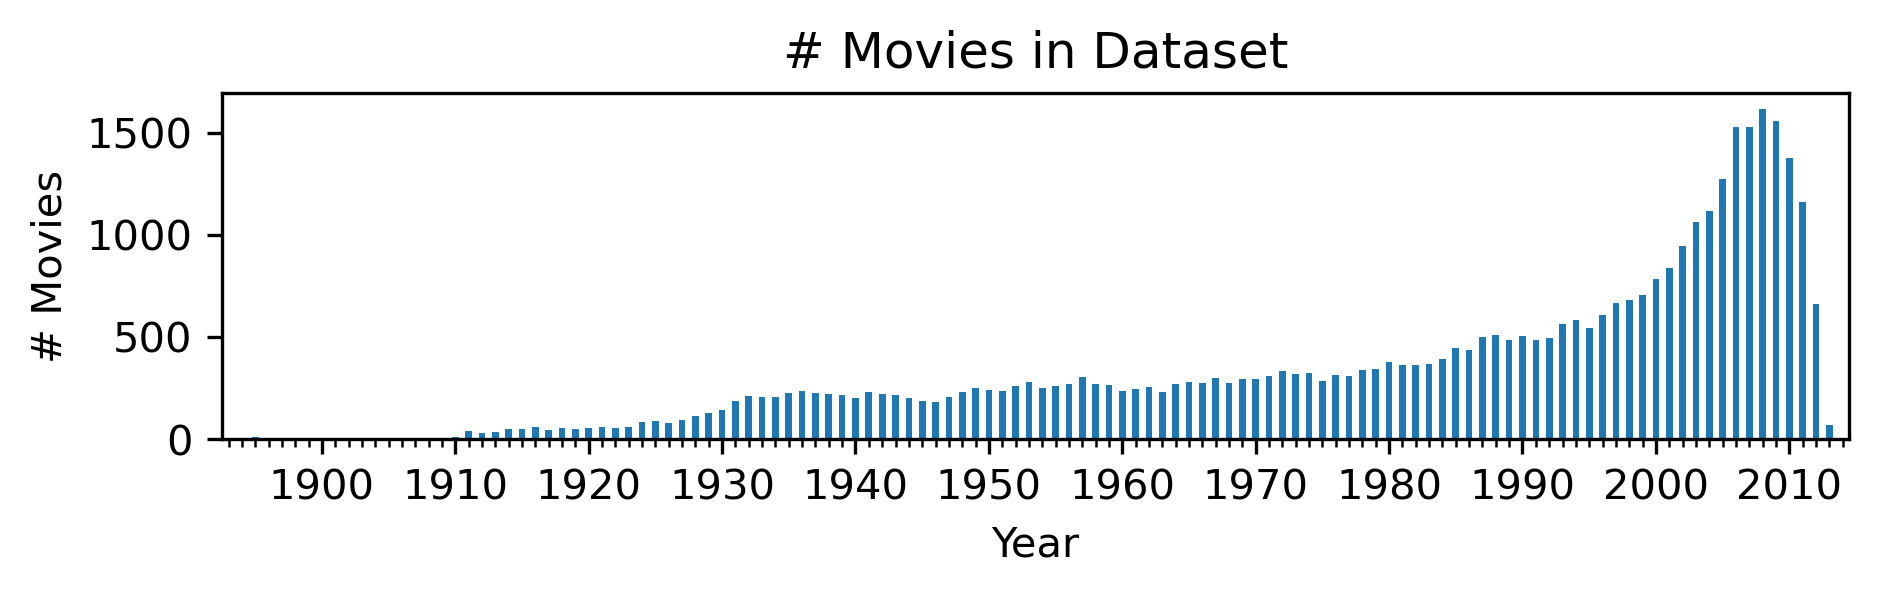
\includegraphics[width=5in]{figures/number_movies_per_year_bar_chart.png}
\label{figure:number_movies_per_year_bar_chart}
\end{figure*}

\begin{table*}
\caption{Dataset variables}
\centering
\begin{tabularx}{.8\textwidth}{llX}
    \textbf{Variable} & \textbf{Description} & \textbf{Example} \\
    \hline
    \texttt{name} & Movie name & \textit{Star Wars Episode IV: A New Hope} \\
    \texttt{date} & Movie release date & \textit{1977-05-25} \\
    \texttt{revenue} & Movie box office revenue (USD) & \textit{775,398,007} \\
    \texttt{runtime} & Movie runtime (minutes) & \textit{122} \\
    \texttt{languages} & Movie languages & \textit{\{English\}} \\
    \texttt{countries} & Movie countries & \textit{\{United States of America\}} \\
    \texttt{genres} & Movie genres & \textit{\{Action, Adventure, Coming-of-age, Family, Fantasy, Science Fiction, Space western\}} \\
    \texttt{summary} & Movie plot summary & \textit{The film begins with an opening crawl explaining that the galaxy is in a state of civil war and that spies for the Rebel Alliance have \ldots} \\
\end{tabularx}
\label{table:variables}
\end{table*}

Although movies can come from different countries and may be in different languages, all of the movie plot summaries are in English (as the dataset is extracted from English Wikipedia).

The variable of focus here is \texttt{summary}, from which we extract key phrases to drive our analysis.

\section{Methods} % How did I approach it?
We first extract key phrases from \texttt{summary} using AutoPhrase \cite{DBLP:journals/corr/ShangLJRVH17}, a phrase mining framework that extracts high-quality phrases from a given text. We use AutoPhrase for its ability to extract high-quality phrases more effectively than traditional, rudimentary, phrase mining techniques, while maintaining minimal human effort during training.

We first train AutoPhrase on all movie plot summaries in the dataset, then extract the key phrases from each individual summary and add these phrases as a variable in our dataset as seen in Table \ref{table:additional_variables}. Figure \ref{figure:key_phrases_example} gives an example of phrases extracted from a movie plot summary by AutoPhrase.

\begin{table*}
\caption{Added variables}
\centering
\begin{tabularx}{.8\textwidth}{llX}
    \textbf{Variable} & \textbf{Description} & \textbf{Example} \\
    \hline
    \texttt{phrases} & Phrases extracted from \texttt{summary} & \textit{\{alderaan, anakin skywalker, assault, aunt and uncle, bay, c-3po, chewbacca, civil war, commanding officer, darth vader, \ldots\}} \\
\end{tabularx}
\label{table:additional_variables}
\end{table*}

\begin{figure*}
\caption{Example of phrases extracted by AutoPhrase}
\begin{quoting}[leftmargin=.1\textwidth]
\small\textit{The \hl{film} begins with an opening crawl explaining that the \hl{galaxy} is in a \hl{state} of \hl{civil war} and that spies for the \hl{Rebel Alliance} have \hl{stolen} plans to the Galactic Empire's \hl{Death Star}, a \hl{heavily armed} and armored \hl{space station} capable of annihilating an \hl{entire planet}. \hl{Rebel leader} \hl{Princess Leia} is in possession of the plans, but her \hl{ship} is captured by Imperial forces under the command of the evil \hl{lord} \hl{Darth Vader}. Before she is captured, \hl{Leia} hides the plans in the \hl{memory} of an astromech droid called \hl{R2-D2} , along with a holographic \hl{recording}. The small droid flees to the surface of the \hl{desert planet} \hl{Tatooine} with \hl{fellow} protocol droid \hl{C-3PO} . The \hl{droids} are quickly captured by\ldots}
\end{quoting}
\label{figure:key_phrases_example}
\end{figure*}

Nearly all extracted phrases are indeed high-quality and encapsulate ideas, events, objects, and characters in the movie plot well.

Our analysis consists of three parts that build off of these extracted phrases:
\begin{enumerate}
    \item An exploratory data analysis (EDA) that examines the progression of human culture over time.
    \item The development and interpretation of a classification model that predicts movie genre.
    \item The development and interpretation of a clustering model that clusters movies.
\end{enumerate}
We expect the combination of these three methods to give us valuable insight into human culture.
\subsection{EDA}
We perform an EDA to discover how human culture and events have progressed over time. Here, we use statistical signals, i.e., tf-idf, to identify when certain phrases (corresponding to discrete entities of human culture and events) are popular and relevant.

We use tf-idf to measure a phrase's relevance in time where each phrase is a term and each period of time (e.g. a year or decade) is a document. We use sublinear term frequency (tf) scaling to reduce the significance of very common phrases (e.g. ``film'', ``life'') that are uninformative in our analysis.

Here, the tf-idf with sublinear tf scaling for a term $t$ of a document $d$ is given by
$$\text{tf-idf}(t, d) = (1 + \log\text{tf}(t, d)) \cdot \left(\log\frac{1 + n}{\text{1 + df}(t)} + 1\right)$$
where $n$ is the total number of documents and $\text{df}(t)$ is the document frequency of $t$.

Given a tf-idf vector for each period of time, we then normalize each tf-idf vector to have a Euclidean norm of 1.

Finally, we define ``top'' phrases as the phrases with the highest tf-idf values for the corresponding period of time.
\subsection{Classification}
\subsection{Clustering}

\section{Results} % What did I find out?
\subsection{EDA}
Figure \ref{figure:top_phrases_by_decade} shows top phrases by decade, where top phrases are defined earlier as the phrases with the highest tf-idf values for the corresponding decade.

\begin{figure*}
\caption{Top phrases by decade, with corresponding highest-grossing movie}
\centering
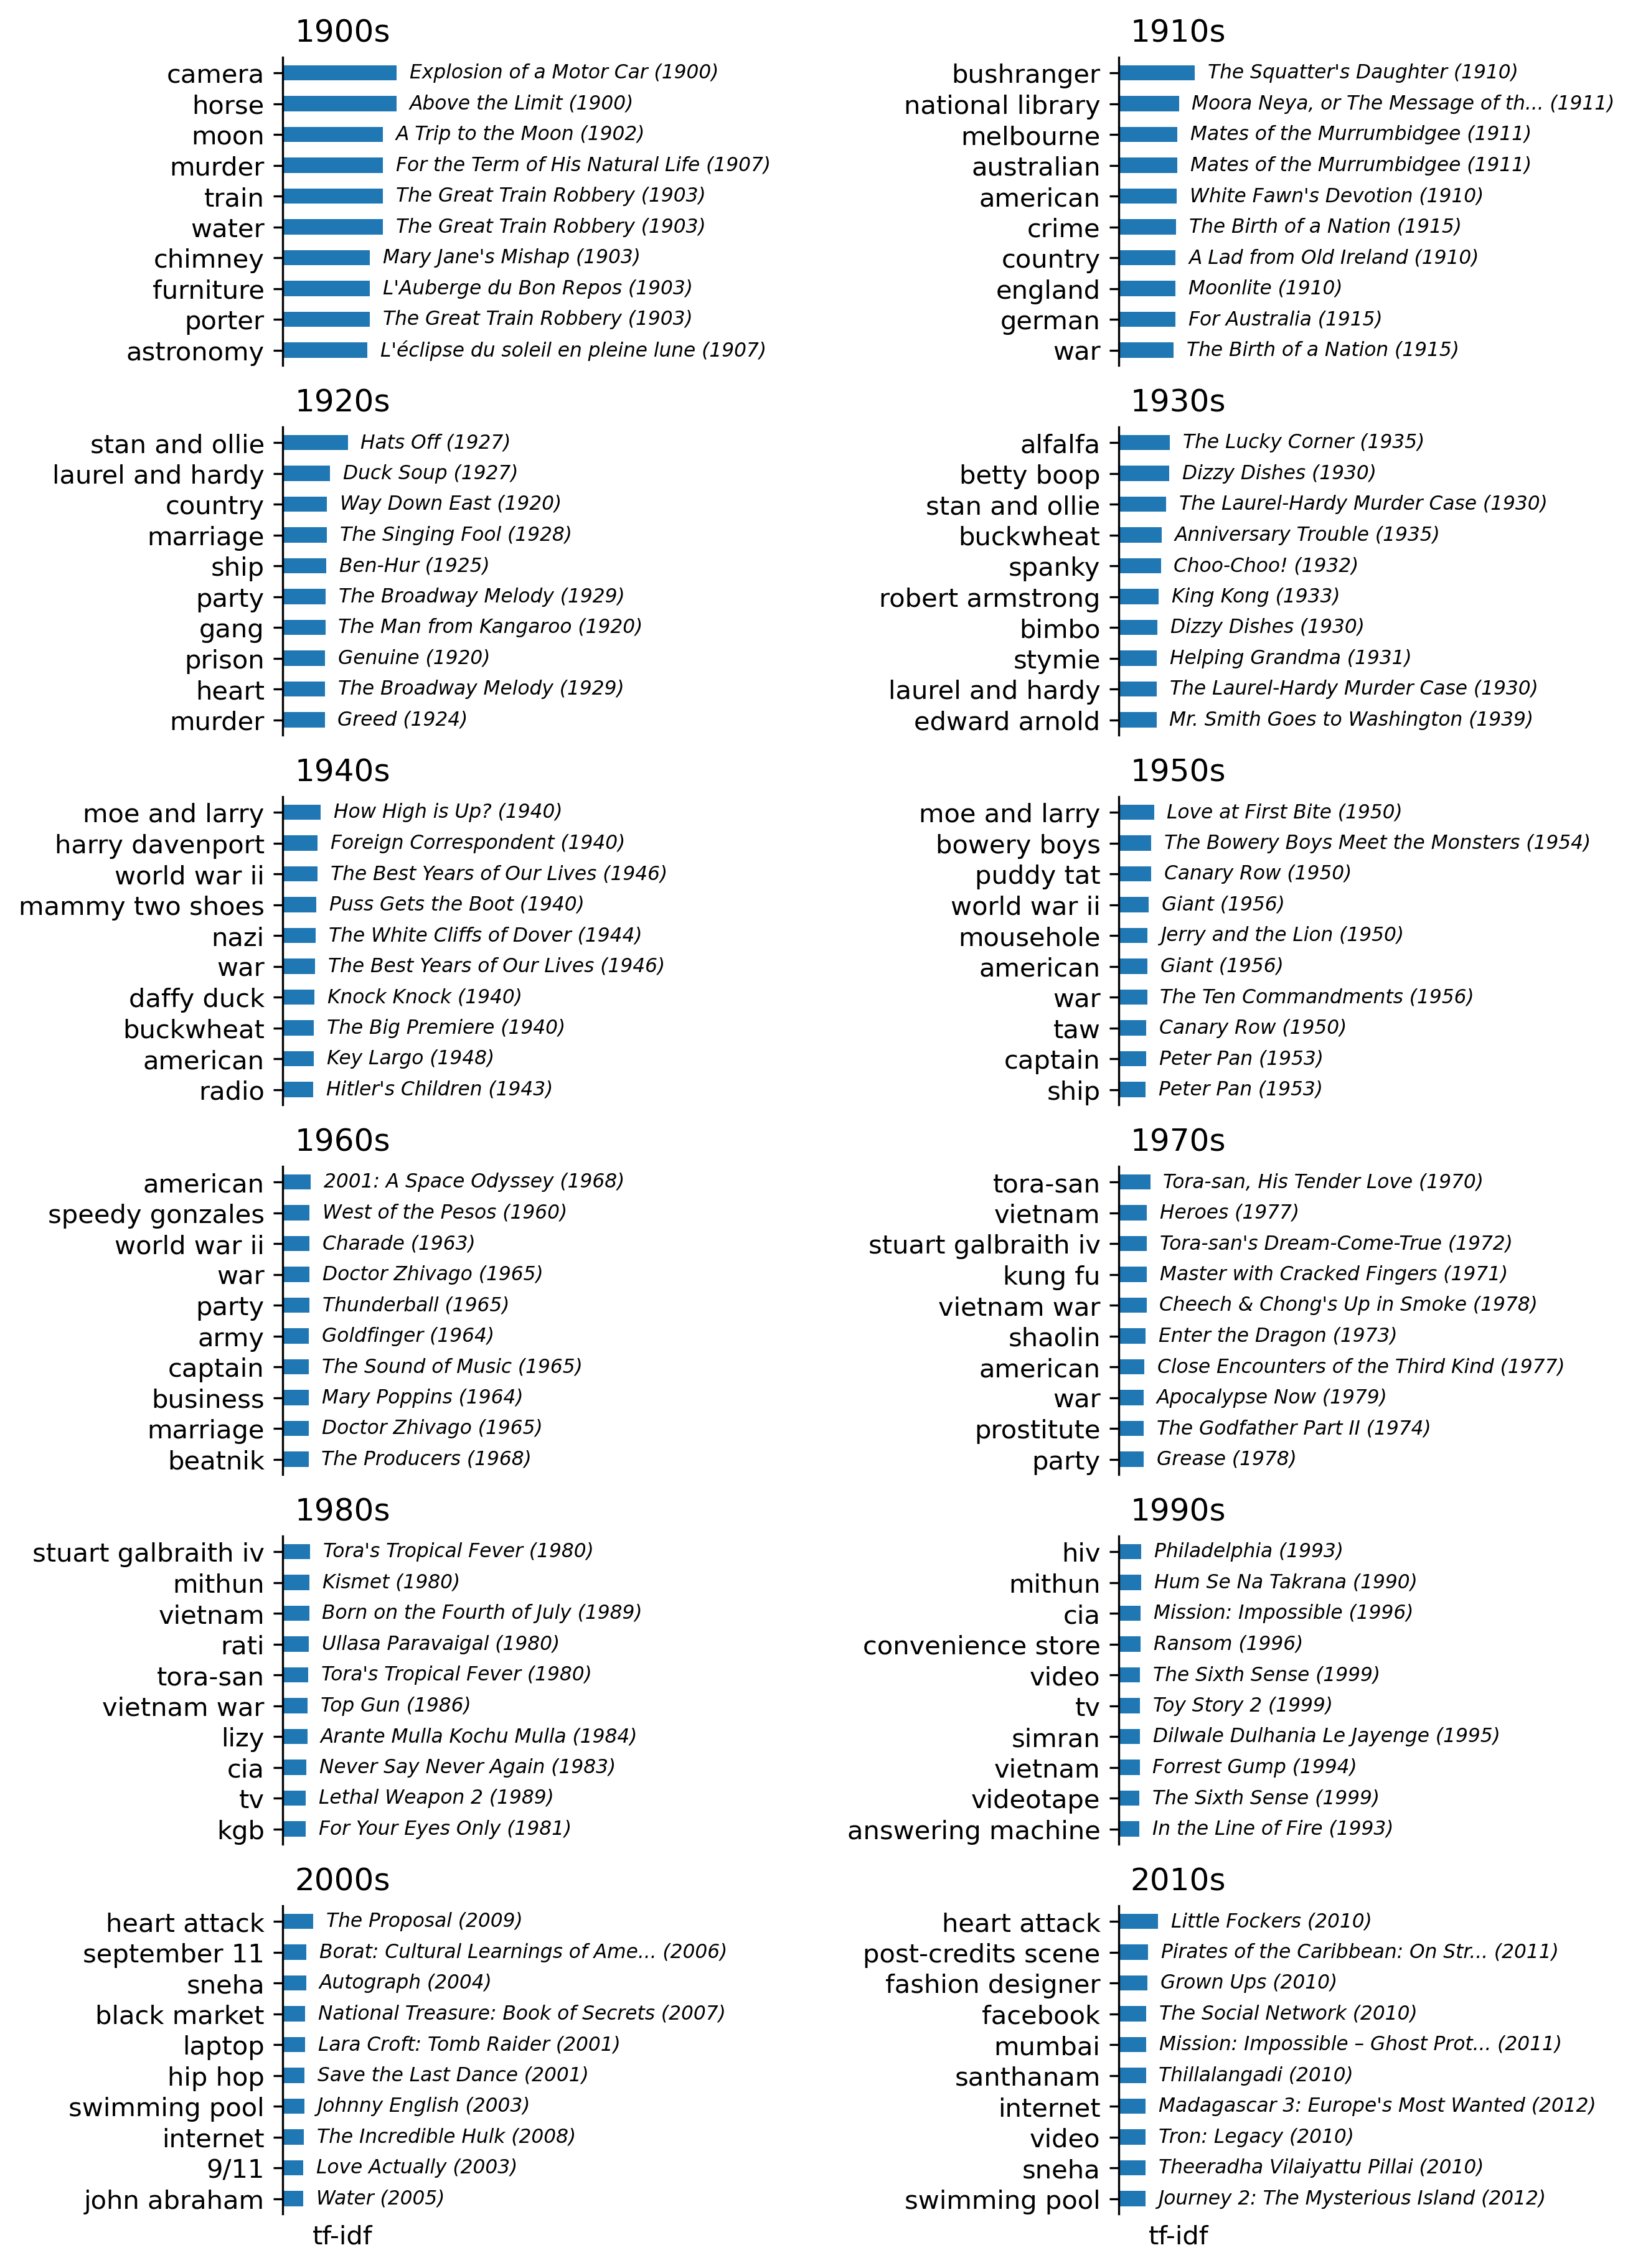
\includegraphics[width=.95\textwidth]{figures/top_phrases_by_decade_bar_chart.png}
\label{figure:top_phrases_by_decade}
\end{figure*}

To provide context, we annotate each phrase with the name and year of the highest-grossing movie out of all movies that contain that phrase in that decade. In the case of a tie in gross revenue, we pick the movie with the earlier release date.

We now examine the results by decade:
\begin{itemize}
    \item \textit{1900s}: It is important to note that the earliest commercial movie screening occurred in 1895 and thus movies were still a relatively new phenomenon in the early 1900s. Top phrases in this decade do not appear to be very salient but do reference objects that may be associated with the early 20th century such as ``horse'' and ``train''.
    \item \textit{1910s}: Many of the top phrases and their corresponding top movies in this decade relate to Australia, which is reasonable since the Commonwealth of Australia was established in 1901 and was a novel setting during this time. This includes the phrases ``bushranger'' (an outlaw living in the Australian bush), ``Melbourne'', and ``Australian'' and the movies \textit{The Squatter's Daughter}, \textit{Moora Neya, or The Message of the Spear}, \textit{Mates from the Murrumbidgee}, \textit{Moonlite}, and \textit{For Australia}.
    \item \textit{1920s}: The most salient top phrases in this decade, ``Stan and Ollie'' and ``Laurel and Hardy'', refer to the internationally famous comedy duo Stan Laurel and Oliver Hardy, whose act was active from the 1920s to 1950s.
    \item \textit{1930s}: We see the appearance of movie characters Alfafa, Buckwheat, Spanky, and Stymie from the \textit{Our Gang} comedy series, Betty Boop and Bimbo from the \textit{Talkartoon} and \textit{Betty Boop} cartoon series, actors Robert Armstrong in \textit{King Kong} and Edward Arnold in \textit{Mr. Smith Goes to Washington}, and the reappearance of Stan and Ollie.
    \item \textit{1940s}: Many of the top phrases and their corresponding top movies in this decade relate to World War II, fought from 1939 to 1945, including the phrases ``World War II'' and ``Nazi'' and the movies \textit{Foreign Correspondent}, \textit{The Best Years of Our Lives}, \textit{The White Cliffs of Dover}, and \textit{Hitler's Children}. We see the appearance of movie characters Mammy Two Shoes from the the \textit{Tom and Jerry} cartoon series, Daffy Duck from the \textit{Looney Tunes} and \textit{Merrie Melodies} cartoon series, actors Moe and Larry, the two mainstay members of The Three Stooges, a famous comedy team active from the 1920s to 1970s (the third stooge changed multiple times throughout the team's history) and Harry Davenport in \textit{Foreign Correspondent}, and the reappearance of Buckwheat.
    \item \textit{1950s}: We continue to see phrases and movies relating to World War II, including the movie \textit{Giant}. We see the appearance of movie characters The Bowery Boys and the reappearance of Moe and Larry. We also see the phrase ``Puddy Tat'' from Tweety's catchphrase ``I Taut I Taw a Puddy-Tat'' from the Sylvester and Tweety cartoons and the phrase ``mousehole'' from the \textit{Tom and Jerry} cartoon series.
    \item \textit{1960s}: We continue to see phrases and movies relating to World War II. We see the use of the phrase ``beatnik'', a media stereotype prevalent from the 1940s to 1960s associated with the nonconformist Beat Generation literary movement in the post-war era, whose elements were later incorporated into the hippie movement and other counterculture movements. We see the appearance of movie characters Speedy Gonzales from the \textit{Looney Tunes} and \textit{Merrie Melodies} cartoon series.
    \item \textit{1970s}: Many of the top phrases and their corresponding top movies in this decade relate to the Vietnam War, fought from 1955 to 1975, including the phrases ``Vietnam'' and ``Vietnam War''. Other top phrases and their corresponding top movies relate to martial arts, including the phrases ``kung fu'' and ``Shaolin''. During this time, martial arts movies rose in popularity, such as those featuring Bruce Lee, which helped lead to an increase in Asian and Asian American representation in cinema. We see the appearance of movie characters Tora-san from the \textit{Otoko wa Tsurai yo} Japanese film series and film historian and critic Stuart Galbraith IV.
    \item \textit{1980s}: We continue to see phrases and movies relating to the Vietnam War. We see the appearance of America's CIA, founded in 1947, and the Soviet Union's KGB, formed in 1954, two opposing security/intelligence agencies whose appearance in movies may have been popularized by the Cold War during this time period. We see the appearance of Indian cinema in the form of actors Mithun Chakraborty in \textit{Kismet}, considered to be one of the foundational films of Bollywood, Lizy in \textit{Arante Mulla Kochu Mulla}, and Rati Agnihotri in \textit{Ullasa Paravaigal}. We see the reappearance of Tora-San and Stuart Galbraith IV.
    \item \textit{1990s}: The top phrase in this decade is ``HIV'', which was first clinically observed in 1981, triggering much of the early HIV/AIDS research in the 1980s. This development may have led to HIV/AIDS being recognized by popular culture in the following years; in fact, the corresponding top movie, \textit{Philadelphia}, was one of the first mainstream Hollywood movies to mention HIV/AIDS. We continue to see phrases and movies relating to the CIA and Vietnam War. We see technologies that may have been more readily accessible to consumers in the late 20th century, such as ``video'', ``tv'', ``videotape``, and ``answering machine''. We see the appearance of movie character Simran Singh in another Bollywood movie, \textit{Dilwale Dulhania Le Jayenge} and the reappearance of Mithun.
    \item \textit{2000s}: The top phrase in this decade is ``heart attack''. It is unclear why, but as a continuously leading cause of death, cardiovascular disease may have found its way into popular culture in this time period. We see top phrases relating to the September 11 attacks, namely ``September 11'' and ``9/11''. We continue to see technologies that are relevant to consumers in this time period, namely ``laptop'' and ``internet``. We see the appearance of ``hip hop'', which became the top-selling music genre by 1999 and continued to become increasingly popular throughout the 2000s. We see the appearance of actors Sneha in \textit{Autograph} and John Abraham in \textit{Water}.
    \item \textit{2010s}: We come to the most recent decade in the dataset. ``Heart attack'' continues to be the top phrase in this decade. We continue to see technologies that are relevant to consumers in this time period, namely ``Facebook'' and ``internet``. Indian cinema continues its presence with the appearance of actor N. Santhanam in \textit{Thillalangadi} and the reappearance of Sneha in \textit{Theeradha Vilaiyattu Pillai}.
\end{itemize}

We can see that examining and researching top phrases over time gives us valuable insight into human culture and its public attitudes, events, people, ideas, etc. Phrase mining and the use of tf-idf automatically identifies relevant keywords in a way that would be difficult to do manually or by using traditional text mining methods.

Figure \ref{figure:top_phrases_by_year} in \nameref{appendix} goes into much finer detail by showing top phrases by year instead of decade and is also available as an \href{https://www.youtube.com/watch?v=8aOob6iJO5Y}{animation}. Here, we observe a similar trend of top phrases across time but also observe phrases that are peculiar to each year.

\subsection{Classification}
\subsection{Clustering}

\section{Discussion} % What did it mean?
In this paper, we apply phrase mining to movie plots, a novel approach for the textual analysis of movies, for a unique insight into human culture.

In the EDA investigation, we use statistical signals to select the most relevant phrases describing each time period. In the classification investigation, \ldots. In the clustering investigation, \ldots.

In each of these investigations, we demonstrate phrase mining's effectiveness in producing valuable insight into human culture.

For future work, we may consider omitting movie character and/or actor names from the top phrases, as movie characters and actors, unless historically significant, are not central to our analysis of human culture.

\bibliographystyle{plain} % Who did I cite?
\nocite{10.1145/2723372.2751523}
\bibliography{report}

\section{Appendix} \label{appendix} % Details!
\begin{figure*}
\caption{Top phrases by year}
\centering
\adjincludegraphics[width=\textwidth,trim=0 {.53\height} 0 0,clip]{figures/top_phrases_by_year_bar_chart.png}
\label{figure:top_phrases_by_year}
\end{figure*}

\begin{figure*}
\ContinuedFloat
\centering
\adjincludegraphics[width=\textwidth,trim=0 0 0 {.47\height},clip]{figures/top_phrases_by_year_bar_chart.png}
\end{figure*}
\end{multicols}

\end{document}
